\documentclass{standalone}
\usepackage{tikz}
\usetikzlibrary{patterns, positioning}
\usepackage[sfdefault]{ClearSans} %% option 'sfdefault' activates Clear Sans as the default text font
\usepackage[T1]{fontenc}

\begin{document}
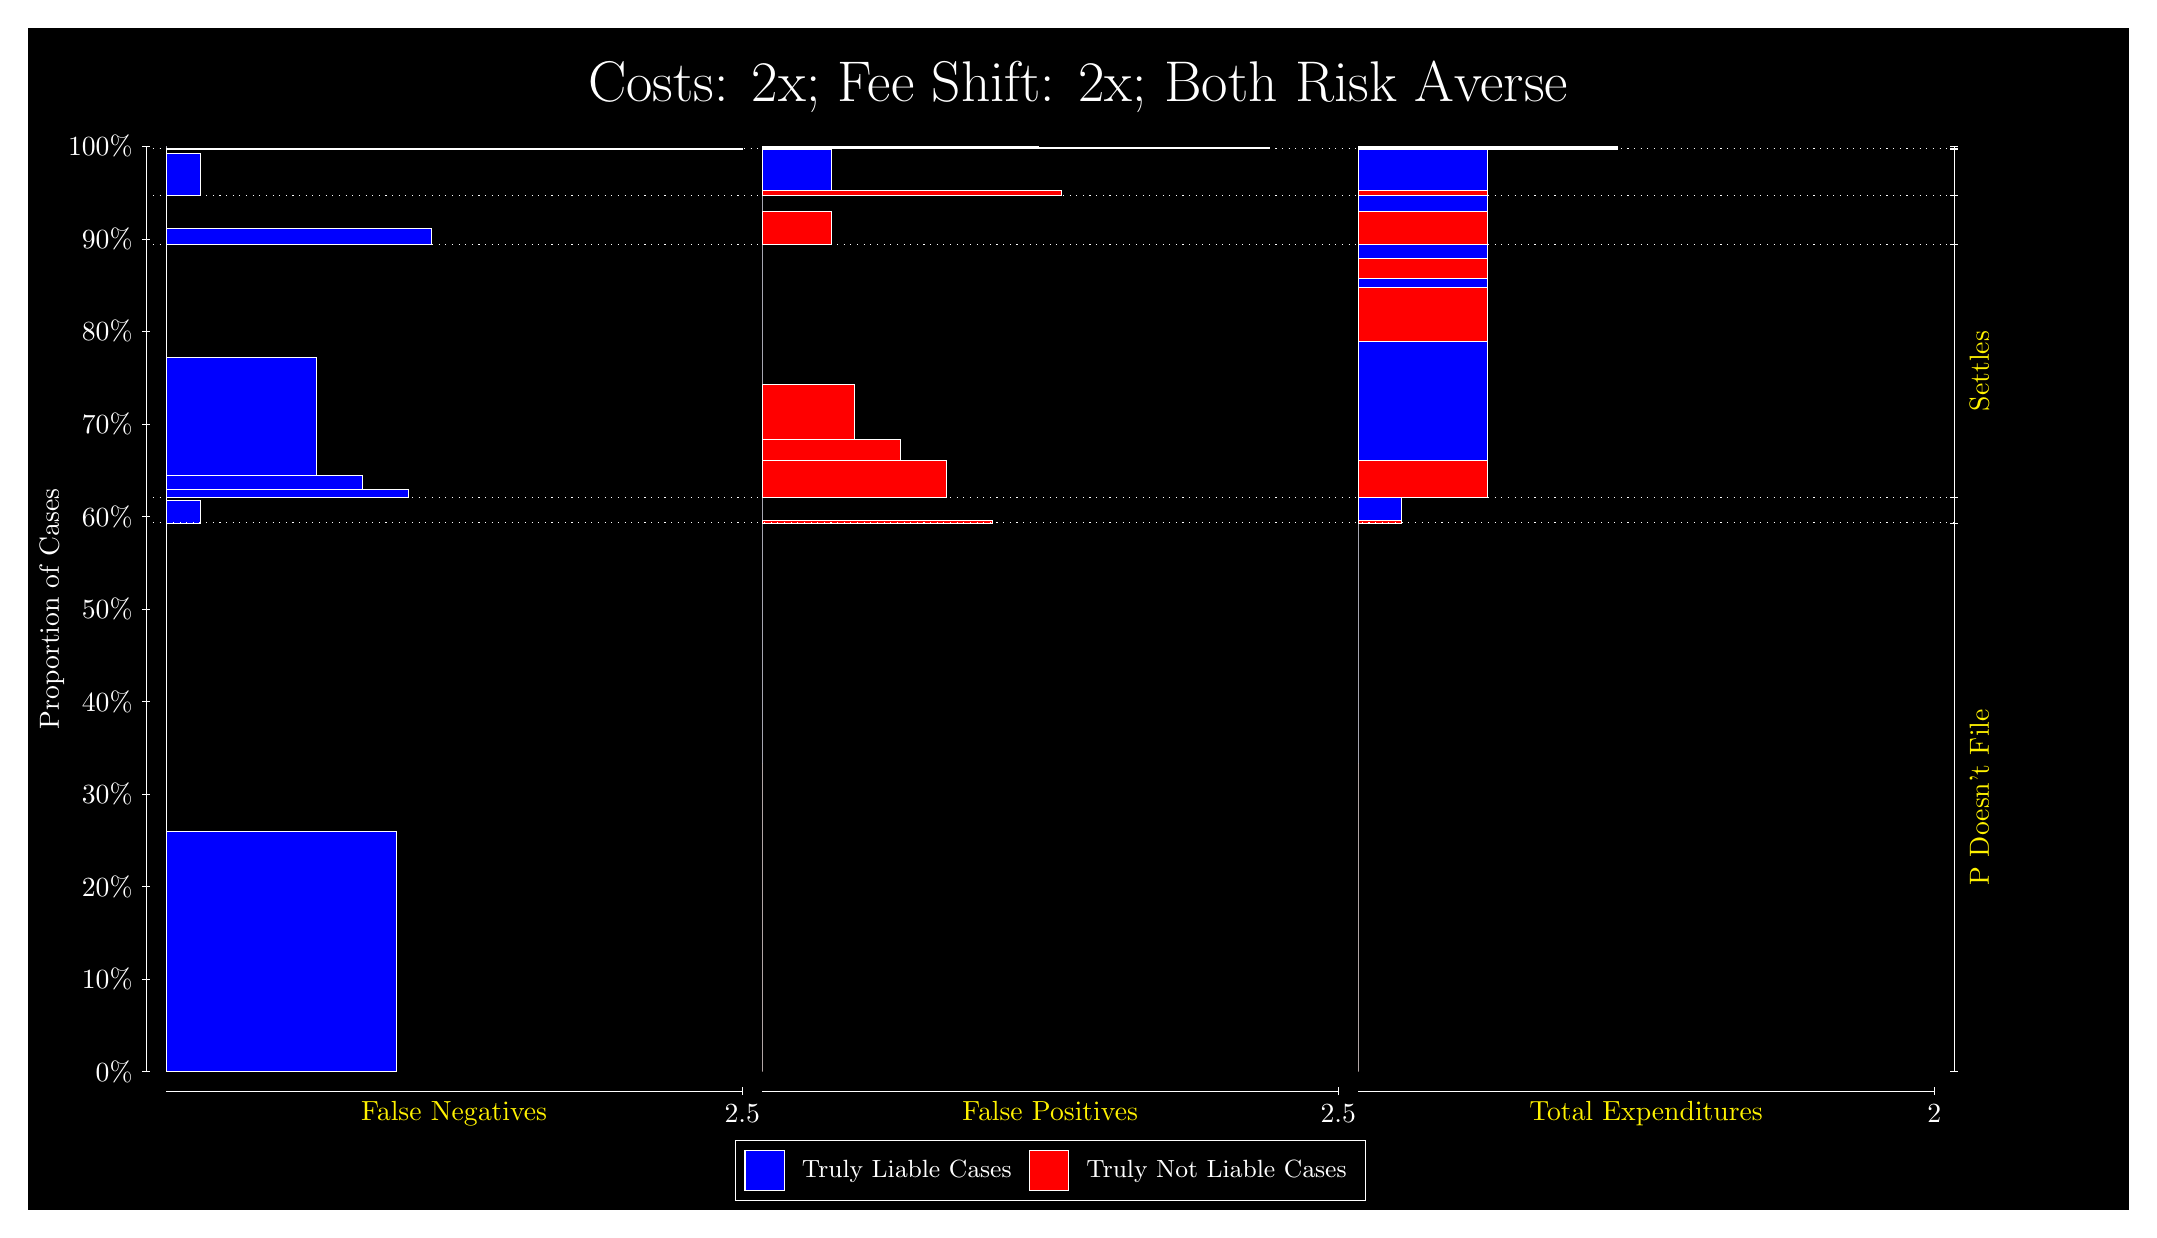
\begin{tikzpicture}
\draw[fill=black] (0,0) rectangle (26.667,15);
\draw[text=white] (0,13.5) rectangle (26.667,15) node[midway] {\huge Costs: 2x; Fee Shift: 2x; Both Risk Averse};
\draw[white, very thin] (1.5,1.75) -- (1.5,13.5);
\node[rotate=90, text=white, anchor=center] at (0.3, 7.625) {Proportion of Cases};
\draw[white, very thin] (1.45,1.75) -- (1.55,1.75);
\node[text=white, anchor=east] at (1.45, 1.75) {0\%};
\draw[white, very thin] (1.45,2.925) -- (1.55,2.925);
\node[text=white, anchor=east] at (1.45, 2.925) {10\%};
\draw[white, very thin] (1.45,4.1) -- (1.55,4.1);
\node[text=white, anchor=east] at (1.45, 4.1) {20\%};
\draw[white, very thin] (1.45,5.275) -- (1.55,5.275);
\node[text=white, anchor=east] at (1.45, 5.275) {30\%};
\draw[white, very thin] (1.45,6.45) -- (1.55,6.45);
\node[text=white, anchor=east] at (1.45, 6.45) {40\%};
\draw[white, very thin] (1.45,7.625) -- (1.55,7.625);
\node[text=white, anchor=east] at (1.45, 7.625) {50\%};
\draw[white, very thin] (1.45,8.8) -- (1.55,8.8);
\node[text=white, anchor=east] at (1.45, 8.8) {60\%};
\draw[white, very thin] (1.45,9.975) -- (1.55,9.975);
\node[text=white, anchor=east] at (1.45, 9.975) {70\%};
\draw[white, very thin] (1.45,11.15) -- (1.55,11.15);
\node[text=white, anchor=east] at (1.45, 11.15) {80\%};
\draw[white, very thin] (1.45,12.325) -- (1.55,12.325);
\node[text=white, anchor=east] at (1.45, 12.325) {90\%};
\draw[white, very thin] (1.45,13.5) -- (1.55,13.5);
\node[text=white, anchor=east] at (1.45, 13.5) {100\%};

\draw[white, very thin] (24.457,1.75) -- (24.457,13.5);
\draw[white, very thin] (24.407,1.75) -- (24.507,1.75);
\node[anchor=west] at (24.407, 1.75) {};
\draw[white, very thin] (24.407,8.7182) -- (24.507,8.7182);
\node[anchor=west] at (24.407, 8.7182) {};
\draw[white, very thin] (24.407,9.0407) -- (24.507,9.0407);
\node[anchor=west] at (24.407, 9.0407) {};
\draw[white, very thin] (24.407,12.253) -- (24.507,12.253);
\node[anchor=west] at (24.407, 12.253) {};
\draw[white, very thin] (24.407,12.878) -- (24.507,12.878);
\node[anchor=west] at (24.407, 12.878) {};
\draw[white, very thin] (24.407,13.467) -- (24.507,13.467);
\node[anchor=west] at (24.407, 13.467) {};
\draw[white, very thin] (24.407,13.478) -- (24.507,13.478);
\node[anchor=west] at (24.407, 13.478) {};
\draw[white, very thin] (24.407,13.5) -- (24.507,13.5);
\node[anchor=west] at (24.407, 13.5) {};

\draw[white, very thin, fill=blue] (1.75,1.75) rectangle (4.6775,4.8025);
\draw[white, very thin, fill=red] (1.75,4.8025) rectangle (1.75,8.7182);
\draw[white, very thin, fill=blue] (1.75,8.7182) rectangle (2.1891,9.0077);
\draw[white, very thin, fill=red] (1.75,9.0077) rectangle (1.75,9.0407);
\draw[white, very thin, fill=blue] (1.75,9.0407) rectangle (4.8239,9.1508);
\draw[white, very thin, fill=blue] (1.75,9.1508) rectangle (4.2384,9.3198);
\draw[white, very thin, fill=blue] (1.75,9.3198) rectangle (3.6529,10.819);
\draw[white, very thin, fill=red] (1.75,10.819) rectangle (1.75,12.253);
\draw[white, very thin, fill=blue] (1.75,12.253) rectangle (5.1167,12.455);
\draw[white, very thin, fill=red] (1.75,12.455) rectangle (1.75,12.878);
\draw[white, very thin, fill=blue] (1.75,12.878) rectangle (2.1891,13.409);
\draw[white, very thin, fill=red] (1.75,13.409) rectangle (1.75,13.467);
\draw[white, very thin, fill=blue] (1.75,13.467) rectangle (9.0689,13.472);
\draw[white, very thin, fill=red] (1.75,13.472) rectangle (1.75,13.478);
\draw[white, very thin, fill=red] (1.75,13.478) rectangle (1.75,13.484);
\draw[white, very thin, fill=blue] (1.75,13.484) rectangle (1.75,13.5);
\draw[white, very thin, fill=red] (9.3189,1.75) rectangle (9.3189,5.6657);
\draw[white, very thin, fill=blue] (9.3189,5.6657) rectangle (9.3189,8.7182);
\draw[white, very thin, fill=red] (9.3189,8.7182) rectangle (12.246,8.7512);
\draw[white, very thin, fill=blue] (9.3189,8.7512) rectangle (9.3189,9.0407);
\draw[white, very thin, fill=red] (9.3189,9.0407) rectangle (11.661,9.5191);
\draw[white, very thin, fill=red] (9.3189,9.5191) rectangle (11.075,9.7794);
\draw[white, very thin, fill=red] (9.3189,9.7794) rectangle (10.49,10.475);
\draw[white, very thin, fill=blue] (9.3189,10.475) rectangle (9.3189,12.253);
\draw[white, very thin, fill=red] (9.3189,12.253) rectangle (10.197,12.676);
\draw[white, very thin, fill=blue] (9.3189,12.676) rectangle (9.3189,12.878);
\draw[white, very thin, fill=red] (9.3189,12.878) rectangle (13.125,12.936);
\draw[white, very thin, fill=blue] (9.3189,12.936) rectangle (10.197,13.467);
\draw[white, very thin, fill=red] (9.3189,13.467) rectangle (9.3189,13.472);
\draw[white, very thin, fill=blue] (9.3189,13.472) rectangle (9.3189,13.478);
\draw[white, very thin, fill=red] (9.3189,13.478) rectangle (15.759,13.484);
\draw[white, very thin, fill=blue] (9.3189,13.484) rectangle (12.832,13.5);
\draw[white, very thin, fill=red] (16.888,1.75) rectangle (16.888,5.6657);
\draw[white, very thin, fill=blue] (16.888,5.6657) rectangle (16.888,8.7182);
\draw[white, very thin, fill=red] (16.888,8.7182) rectangle (17.437,8.7512);
\draw[white, very thin, fill=blue] (16.888,8.7512) rectangle (17.437,9.0407);
\draw[white, very thin, fill=red] (16.888,9.0407) rectangle (18.534,9.5191);
\draw[white, very thin, fill=blue] (16.888,9.5191) rectangle (18.534,11.018);
\draw[white, very thin, fill=red] (16.888,11.018) rectangle (18.534,11.714);
\draw[white, very thin, fill=blue] (16.888,11.714) rectangle (18.534,11.824);
\draw[white, very thin, fill=red] (16.888,11.824) rectangle (18.534,12.084);
\draw[white, very thin, fill=blue] (16.888,12.084) rectangle (18.534,12.253);
\draw[white, very thin, fill=red] (16.888,12.253) rectangle (18.534,12.676);
\draw[white, very thin, fill=blue] (16.888,12.676) rectangle (18.534,12.878);
\draw[white, very thin, fill=red] (16.888,12.878) rectangle (18.534,12.936);
\draw[white, very thin, fill=blue] (16.888,12.936) rectangle (18.534,13.467);
\draw[white, very thin, fill=red] (16.888,13.467) rectangle (20.181,13.472);
\draw[white, very thin, fill=blue] (16.888,13.472) rectangle (20.181,13.478);
\draw[white, very thin, fill=red] (16.888,13.478) rectangle (20.181,13.484);
\draw[white, very thin, fill=blue] (16.888,13.484) rectangle (20.181,13.5);
\draw[white, dotted] (1.5,8.7182) -- (24.457,8.7182);
\draw[white, dotted] (1.5,9.0407) -- (24.457,9.0407);
\draw[white, dotted] (1.5,12.253) -- (24.457,12.253);
\draw[white, dotted] (1.5,12.878) -- (24.457,12.878);
\draw[white, dotted] (1.5,13.467) -- (24.457,13.467);
\draw[white, dotted] (1.5,13.478) -- (24.457,13.478);
\draw[white, very thin] (1.75,1.5) -- (9.0689,1.5);
\node[text=yellow, anchor=north] at (5.4094, 1.5) {False Negatives};
\draw[white, very thin] (9.0689,1.45) -- (9.0689,1.55);
\node[text=white, anchor=north] at (9.0689, 1.45) {2.5};

\draw[white, very thin] (9.3189,1.5) -- (16.638,1.5);
\node[text=yellow, anchor=north] at (12.978, 1.5) {False Positives};
\draw[white, very thin] (16.638,1.45) -- (16.638,1.55);
\node[text=white, anchor=north] at (16.638, 1.45) {2.5};

\draw[white, very thin] (16.888,1.5) -- (24.207,1.5);
\node[text=yellow, anchor=north] at (20.547, 1.5) {Total Expenditures};
\draw[white, very thin] (24.207,1.45) -- (24.207,1.55);
\node[text=white, anchor=north] at (24.207, 1.45) {2};

\node[text=yellow, centered, rotate=90] at (24.777, 5.2341) {P Doesn't File};

\node[text=yellow, centered, rotate=90] at (24.777, 10.647) {Settles};





\draw (12.978300999999998,1.5) node[draw=none] (baseCoordinate) {};
\begin{scope}[align=center]
        \matrix[scale=0.5, draw=white, below=0.5cm of baseCoordinate, nodes={draw}, column sep=0.1cm]{
            \node[rectangle, draw, minimum width=0.5cm, minimum height=0.5cm, fill=blue] {}; &
            \node[draw=none, font=\small, text=white] (B) {Truly Liable Cases}; &
            \node[rectangle, draw, minimum width=0.5cm, minimum height=0.5cm, fill=red] {}; &
            \node[draw=none, font=\small, text=white] (B) {Truly Not Liable Cases}; \\
            };
\end{scope}

\end{tikzpicture}
\end{document}